\section{Crypt$\epsilon$ Implementation }
\subsection{\system Primitives Implementation}
1) \textbf{\textsf{CrossProduct}}($\tilde{\mathbf{T}}, A_i, A_j$): Let $D_1$ and $D_2$  be the encrypted one-hot-coding corresponding to two  values $v_1$ and $v_2$ (integral representation) for attributes $A_1$ and $A_2$ respectively. The corresponding encrypted one-hot-encoding for the two-dimensional attribute $A_1\times A_2$ is given by  \begin{gather} D_{1\times 2}[(i-1)\cdot s_{A_2}+j] = labMult(D_1[i], D_2[j])\\ i \in [s_{A_1}], j \in [s_{A_2}]\end{gather} For this particular case, only $D_{1 \times 2}[(v_1-1)\cdot s_{A_2}+v_2]=Enc(1)$ while all other indices will equate to $Enc(0)$. Note that when computing the one-hot-encoding for a t-dimensional attribute $t > 2$,  for the actual implementation, instead of calling $t$ iterative instances of \textsf{CrossProduct}() we use the $genLabMult()$ operator of labeled homomorphic encryption to speed up the computation. 
2) \textbf{\textsf{Project}}($\tilde{\mathbf{T}}, A^*$)- The implementation of the \textsf{Project} transformation is very straightforward, it simply drops off all but the attributes in $A^*$ from $\tilde{\mathbf{T}}$ and returns the truncated table.

3)\textbf{ \textsf{Filter}}($\mathbf{\tilde{T}},\phi$)-  As discussed in the preceding section, the predicate $\phi$ is expressed in a special form of conjunctions of range conditions given by eq \ref{phi}. Now for a range condition $A \in \{v_1,...v_t\}$, assuming $\mathbf{\tilde{R}_A}[i]$ is the corresponding one-hot-coding for the $i^{th}$ record's value for attribute $A$,  consider the following \begin{gather}\mathbf{c}_A^i=\bigoplus_{j=1}^{t}\tilde{\mathbf{R}}_{A}[i][v_1]\end{gather} where $\tilde{\mathbf{R}}_{A}[i][v]$ is the $v^{th}$ index of corresponding one-hot-coding. Clearly if the $i^{th}$ record satisfies the condition $A \in \{v_1,...v_t\}$, then exactly one of the values in $\{\tilde{\mathbf{R}}_{A}[i][v_j]\}, j \in \{1,...,t\}$ will be a cipher for $1$. Thus $c_A^i=1$ if record $i$ satisfies the range condition and 0 otherwise. If the condition is instead an equality predicate $A==v$ then $\mathbf{c}_A^i=\tilde{\mathbf{R}}_{A}[i][v]$. Now considering $\phi$ is given by eq \ref{phi}, let us define\begin{gather}\mathbf{c}^i=genLabMult(\mathbf{c}^i_{A_1},...,\mathbf{c}^i_{A_r})\\A^*=\bigcup_{j=1}^rA_j\end{gather} It is easy to see that $c^i$=1 iff record $i$ satisfies $\phi$. Let $\mathbf{B}'$ be the indicator vector before the execution of the current instance of the \textsf{Filter} transformation. The final step is to multiply the $\mathbf{c}^i$s with the corresponding indicator bits and obtain the updated indicator vector $\mathbf{B}$ as follows \begin{gather}\mathbf{B}[i]=labMult(\mathbf{c}^i,\mathbf{B}'[i])\end{gather} 
The above step zeros out some additional records which were found to be extraneous by some preceding filter conditions. Clearly $\textbf{B}$ is the output of the \textsf{Filter} transformation.
\\\textbf{Avoid Indicator Vector Multiplication}\\
When the \textsf{Filter} transformation is applied for the very first time in a Crypt$\epsilon$ program and the input predicate is conditioned on a single attribute $A \in \{v_1,...,v_k\}$, then we can do the following optimization. Consider \begin{gather}\mathbf{b}[i]=\bigoplus_{j=1}^k \mathbf{\tilde{R}}_A[i][v_j], i \in [m]\end{gather} where $\mathbf{\tilde{R}}_A[i]$ is the one-hot-coding for attribute $A$ for the $i^{th}$ record. Since this is the first instance of the \textsf{Filter} primitive, the current indicator vector $\mathbf{B}$  will be all 1-vector. Thus $\mathbf{b}$ is itself the updated indicator vector  and we can avoid the unnecessary multiplication $labMult(\mathbf{b[i]},\mathbf{B}[i])$.  

4) \textbf{\textsf{Count}}($\mathbf{\hat{T}}$) - The \textsf{Count} primitive takes the associated bit vector $\mathbf{B}$ of its input table $\encT$  and simply adds up its entries to return  \begin{gather}\mathbf{c}=\bigoplus_{i=1}^m\mathbf{B}[i]\end{gather}%\item GroupBy*($\mathbf{V},sk$)- This primitive is an extension of the previous GroupBy transformation. 
5) \textsf{GroupBy*}($\mathbf{\tilde{T}},A$) - The \textsf{GroupBy*} transformation   makes use of three other transformations \textsf{Project, Filter} and \textsf{Count} and is implemented as follows
\begin{enumerate}[label=\alph*)] \item $\mathbf{\tilde{T}}_1$=\textsf{Project}($\mathbf{\tilde{T}}$, $A$) \item $\mathbf{B}$ =  current indicator bit vector \item  for $i = 1:s_A $ \\Intialize bit vector to $\mathbf{B}$  \\$\phi_i= (A==v_{i,A}) $ \\$\hat{\mathbf{T_2}}$ = \textsf{Filter}($\mathbf{\tilde{T}}_1, \phi_i$)\\ $\mathbf{C}[i]$ = \textsf{Count}($\hat{\mathbf{T_2}}$) \\ end for \item Output $\mathbf{C}$ 
\end{enumerate}
6) \textsf{CountDistinct}($\mathbf{V},\epsilon$) - The \textsf{CountDistinct} primitive is implemented as follows \begin{enumerate}[label=\alph*)]\item Firstly the \textsf{AS} creates a mask vector drawn uniformly at random from $[m]^{s_A}$, i.e.,  \begin{gather*} M[i] \in_R [m], i \in [|V|]\end{gather*} \item \textsf{AS} masks the encrypted true count vector $\mathbf{V}$  as follows \begin{gather*}\boldsymbol{\mathcal{V}}[i]= \mathbf{V}[i] \oplus labEnc_{pk}(M[i])\end{gather*} and sends it to the \textsf{CSP} \item \textsf{CSP} decrypts the masked encrypted vector as \begin{gather*}\mathcal{V}[i]=labDec_{sk}(\mathbf{V}[i]), i \in [|V|]\end{gather*} \item Next the \textsf{CSP} generates the following garbled circuit that\begin{enumerate}[label=\roman*)]  \item takes the mask $M$ as an input from the \textsf{AS} \item takes a random number $r$  as an input from the \textsf{CSP}\item takes the decrypted masked vector $\mathcal{V}$ as an input from the \textsf{CSP} \item removes the mask $M$ from $\mathcal{V}$ as \begin{gather*}V[i]=\mathcal{V}[i]-M[i], i \in [|V|]\end{gather*}\item  counts the number of non-zero entries of $V$ as C \item adds the laplace noises \begin{gather*}\mathcal{C}=C+r\end{gather*} and returns $\mathcal{C}$ \end{enumerate} \item The \textsf{AS} evaluates the above circuit and gets output $\mathcal{C}$ \item The \textsf{AS} gets $labEnc_{pk}(r)$ from the \textsf{CSP} and generates $labEnc_{pk}(\mathcal{C})$ to compute\begin{gather*}\mathbf{C}=labEnc_{pk}(\mathcal{C})-labEnc_{pk}(r)\end{gather*} \end{enumerate} 

8) \textsf{Laplace}($\mathbf{V},\epsilon$)- Recall that both \textsf{AS} and \textsf{CSP} have to add Laplace noise to the output in Crypt$\epsilon$. Hence the \textsf{Laplace} primitive has two components. The first component is executed by the \textsf{AS} wherein,
\begin{enumerate} \item \textsf{AS} generates a noisy vector $\eta$ such that $\eta \in [Lap(\frac{1}{\epsilon})]^{|V|}$ \item encrypts $\eta$ and adds it to the input vector as \begin{gather*}\boldsymbol{\eta}=labEnc_{pk}(\eta)\\\mathbf{\hat{V}}[i]=\mathbf{V}[i]\oplus \boldsymbol{\eta}[i], i \in [|V|]\end{gather*} \end{enumerate} This encrypted noisy vector $\mathbf{\hat{V}}$ is the input for the second phase of the \textsf{Laplace} primitive which is executed by the \textsf{CSP} as follows \begin{enumerate}\item Decrypts $\mathbf{\hat{V}}$ \begin{gather*}\hat{V}=labDec_{sk}(\mathbf{\hat{V}})\end{gather*}  \item Generates a noisy vector $\eta'$ such that $\eta' \in [Lap(\frac{1}{\epsilon})]^{|\hat{V}|}$ \item Finally adds the noise $\eta'$ to $\hat{V}$ \begin{gather*}\hat{\mathcal{V}}[i]=\hat{V}[i]+\eta'[i], i \in [|\hat{V}|]\end{gather*} \item Returns $\hat{\mathcal{V}}$ to \textsf{AS} \end{enumerate} 
% Note that in the Crypt$\epsilon$ implementation we need to add two instances of the Laplace noise as opposed to a single instance in the standard central differential privacy setting. After the addition of the first instance of the laplace noise, $\eta$ (by the AS),  the encrypted answer is sent to the CSP. becuse of CSP has only a differential private view Hence the addition of the second instance of the laplace noise can be looked upon as a post-processing step  However and differential privacy is immune to post processing 

9)\textsf{NoisyMax}($\mathbf{V},\epsilon,k$)- The input to the NoisyMax primitive is an encrypted vector $\mathbf{V}$ where each entry $V[i]$ is a count. The primitive is implemented via the following steps.  \begin{enumerate}
\item First the \textsf{AS} adds noise to the input encrypted vector as follows \begin{gather*} \eta \in [Lap(\frac{1}{\epsilon})]^{|V|}\\\boldsymbol{\eta}=labEnc_{pk}(\eta)\\\mathbf{\hat{{V}}}[i]=\mathbf{V}[i]+ \boldsymbol{\eta}[i], i \in [|V|] \end{gather*} \item Next the \textsf{AS} creates a mask vector $M$ drawn uniformly at random from $[m]^{s_A}$, i.e.,  \begin{gather*} M[i] \in_R [m], i \in [|V|]\end{gather*} \item \textsf{AS} masks the encrypted noisy vector $\mathbf{\hat{V}}$  as follows \begin{gather*}\boldsymbol{\mathcal{V}}[i]= \mathbf{\hat{V}}[i] \oplus labEnc_{pk}(M[i]), i \in [|V|]\end{gather*} and sends it to the \textsf{CSP} \item \textsf{CSP} decrypts the masked encrypted noisy vector as \begin{gather*}\mathcal{V}[i]=labDec_{sk}(\mathbf{\hat{V}}[i]), i \in [|V|]\end{gather*} \item Next, the following garbled circuit is evaluated which
    \begin{enumerate}[label=\roman*]\item takes noisy masked  vector $\mathcal{V}$ as an input from the \textsf{CSP} \item takes mask $M$ as the input from \textsf{AS}  \item removes the mask from  $\mathcal{V}$  as \begin{gather*} \hat{V}[i]=\mathcal{V}[i]-M[i], i \in [|V|]\end{gather*}  \item computes the top $k$ element over  $\hat{V}$ and returns $arg_{\textit{top k}}\max{\hat{V}[i])}$
    \end{enumerate}
    \end{enumerate}
 \subsection{DP Index Optimization Implementation}\label{index-imp}
 The DP index optimization can be implemented via a garbled circuit that \begin{enumerate}\item takes the entire database $\boldsymbol{\mathcal{\tilde{D}}}$ as an input and the attribute $A$ as an input from the \textsf{AS}.
\item takes the secret key $sk$ as an input from  the \textsf{CSP} \item Decrypts $\boldsymbol{\mathcal{\tilde{D}}}$ \item Sorts the decrypted database on $A$, i.e., the first $ct_{A,v_1}$ rows are the ones with value $v_1$ for attribute $A$, the next $ct_{A,v_2}$ are  the records with value $v_2$ for attribute $A$ and so on. \item  re-encrypts the sorted database \item Divide the domain of $A$ into $k$ bins such that each bin contains $s_A/k$ consecutive domain values. \item Construct a $k$ lengthed vector $\hat{V}$ such that $\hat{V}[i]=\sum_jct_{A,j}+\eta_i, i \in [k], j \in [\frac{s_A}{k}(i-1)+1,\frac{s_A}{k}i]$ where $\eta_i$ is a random laplace noise drawn from the distribution $Lap(\frac{k}{\epsilon})$ \item Return $\hat{V}$ and sorted $\boldsymbol{\mathcal{\tilde{D}}}_{sort}$\end{enumerate}
\begin{figure}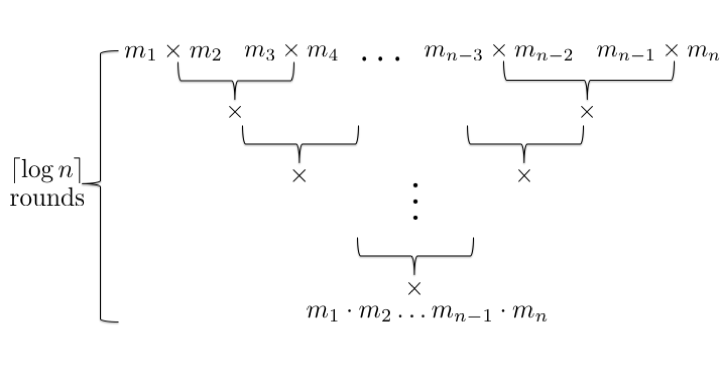
\includegraphics[height=4cm,width=8cm]{kk.png} \caption{ $genLabMult()$ - Batching of multiplicands for \textsf{labHE}} \label{genlab-fig}\end{figure}